\documentclass[a4paper]{article}
\usepackage{amsmath, amssymb, bm}
\usepackage[margin=1in]{geometry}
\usepackage{graphicx}
\begin{document}
\begin{titlepage}
  \centering
    {\huge \bf Assignment 1\par}
    \vspace{1cm}
    {\Large Computational Intelligence, SS2018\par}
    \vspace{1cm}
    \begin{tabular}{|l|l|l|}
      \hline
      \multicolumn{3}{|c|}{\textbf{Team Members}}   \\ \hline
      Last name & First name & Matriculation Number \\ \hline
      Lee       & Eunseo     & 11739623             \\ \hline
      Shadley   & Alex       & 11739595             \\ \hline
      Lee       & Dayeong    & 11730321             \\ \hline
    \end{tabular}
\end{titlepage}

\section{Linear Regression}
\subsection{Derivation of Regularized Linear Regression}
\begin{itemize}
  \item Preliminary questions
    \begin{itemize}
      \item for each i, \(\bm{X}^{(i)}\) is n+1 dimensional column vector. For
        notaion convenience, all \(\bm{X}_0^{(i)}\) is set to \(0\).
      \item The gradient of \(J(\bm{\theta})\) is \[
          \frac{\partial J(\bm{\theta})}{\partial \bm{\theta}} = \langle
          \frac{\partial J(\bm{\theta})}{\partial \theta_0}, \quad
          \frac{\partial J(\bm{\theta})}{\partial \theta_1}, \quad
          \cdots, \quad
          \frac{\partial J(\bm{\theta})}{\partial \theta_n}
          \rangle
        \]. It is n+1 dimensional column vector.
      \item In gradient, function \(f\) is
        \(\mathbb{R}^n\rightarrow\mathbb{R} \) and the gradient itself is vector.
        The jacobian matrix of function
        \(\bm{f}\colon\mathbb{R}^n\rightarrow\mathbb{R}^m\) is
        \[[
          \quad \frac{\partial \bm{f}}{\partial x_1} \quad
          \frac{\partial \bm{f}}{\partial x_2} \quad
          \cdots \quad \frac{\partial \bm{f}}{\partial x_n} \quad
          ] =
          \begin{bmatrix}
            \frac{\partial f_1}{\partial x_1} & \cdots & \frac{\partial f_1}{\partial x_n} \\
            \vdots & \ddots & \vdots \\
            \frac{\partial f_m}{\partial x_1} & \cdots & \frac{\partial f_m}{\partial x_n}
          \end{bmatrix}
          \]
          where \(\bm{f} = <f_1, f_2, \cdots, f_m>\) and \(\bm{x} = <x_1, x_2, \cdots, x_n>\).
          When \(m=0\), Jacobian matrix and gradient are same.
        \item \(\bm{X\theta}\) is \(m\) dimension vector. The dimension of jacobian
          matrix \(\frac{\partial \bm{X\theta}}{\partial \bm{\theta}}\) is \(n+1 \times m\).
          In this case, \(\frac{\partial \bm{X\theta}}{\partial \bm{\theta}}\) is same with \(\bm{X}\).
    \end{itemize}
  \item 2
  \item 3
\end{itemize}

\subsection{Linear Regression with polynomial features}

The following plots demonstrate the results of Linear Regression with polynomial degrees of 1, 2, 5, and 20:

\noindent
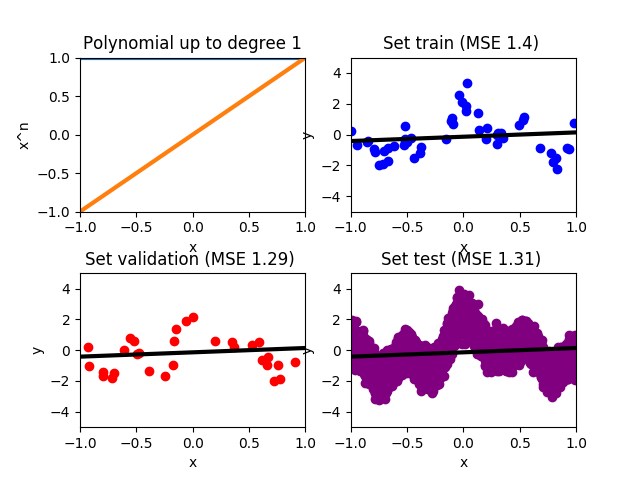
\includegraphics[width=0.5\textwidth]{linreg_deg1.png}%
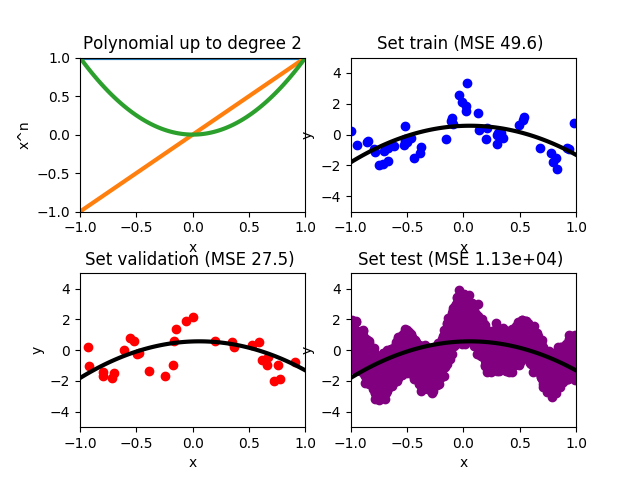
\includegraphics[width=0.5\textwidth]{linreg_deg2.png}\\[2em]
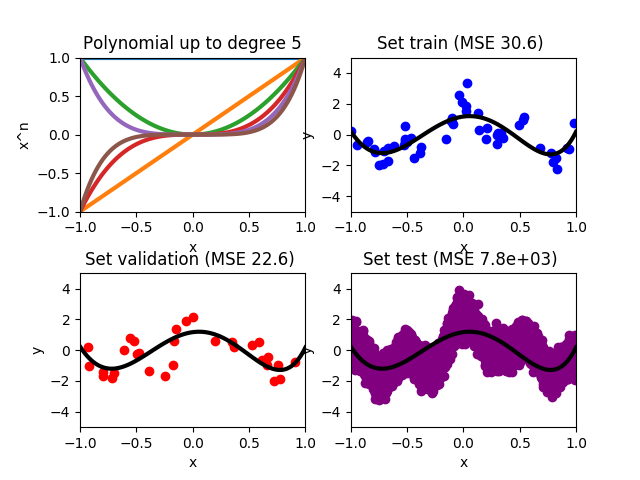
\includegraphics[width=0.5\textwidth]{linreg_deg5.png}%
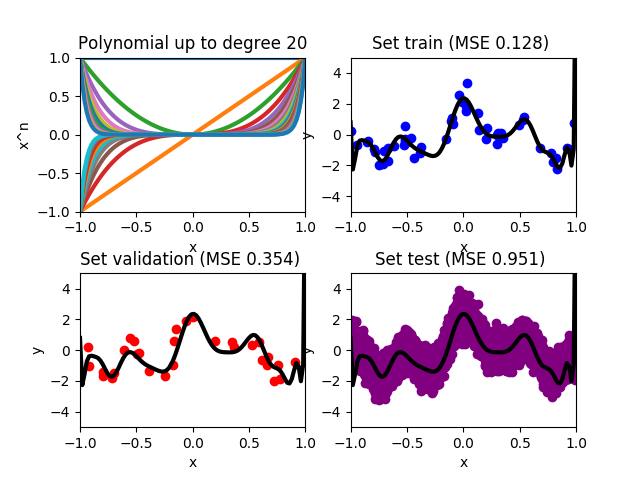
\includegraphics[width=0.5\textwidth]{linreg_deg20.png}\par

\section{Logistic Regression}
\subsection{Derivation of Gradient}
\begin{equation}
  \begin{split}
    J(\bm{\theta}) &= -\frac{1}{m} \sum_{i=1}^{m} \left( y^{(i)} \log (h_{\bm{\theta}}(\bm{x}^{(i)}))
    + (1-y^{(i)} ) \log (1 - h_{\bm{\theta}}(\bm{x}^{(i)}))  \right) \\
    &=  -\frac{1}{m} \sum_{i=1}^{m} \left( y^{(i)} \log (\sigma(\bm{x}^{(i)T}\bm{\theta}))
    + (1-y^{(i)} ) \log (1 - \sigma(\bm{x}^{(i)T}\bm{\theta})  \right)
  \end{split}
\end{equation}
The partial derivative of the cost function with respect $\theta_j$ is
\begin{equation}
  \begin{split}
    \frac{\partial J(\bm{\theta})}{\partial \theta_j }
    &= -\frac{1}{m} \sum_{i=1}^m \left(
    y^{(i)} \frac{1}{\sigma(\bm{x}^{(i)T}\bm{\theta})} \frac{\partial \sigma(\bm{x}^{(i)T}\bm{\theta})}{\partial \theta_j}
    - (1-y^{(i)}) \frac{1}{1-\sigma(\bm{x}^{(i)T}\bm{\theta})} \frac{\partial \sigma(\bm{x}^{(i)T}\bm{\theta})}{\partial \theta_j}
    \right) \\
    &= -\frac{1}{m} \sum_{i=1}^m \left(
    y^{(i)} \frac{\sigma(\bm{x}^{(i)T}\bm{\theta}) \cdot (1 - \sigma(\bm{x}^{(i)T}\bm{\theta}))}{\sigma(\bm{x}^{(i)T}\bm{\theta})} \cdot \frac{\partial \bm{x}^{(i)T}\bm{\theta}}{\partial \theta_j}
    - (1 - y^{(i)}) \frac{\sigma(\bm{x}^{(i)T}\bm{\theta}) \cdot (1 - \sigma(\bm{x}^{(i)T}\bm{\theta}))}{1 - \sigma(\bm{x}^{(i)T}\bm{\theta})} \cdot \frac{\bm{x}^{(i)T}\bm{\theta}}{\partial \theta_j}
    \right) \\
    &= -\frac{1}{m} \sum_{i=1}^{m} \left(
    y^{(i)} \frac{\sigma(\bm{x}^{(i)T}\bm{\theta}) \cdot (1 - \sigma(\bm{x}^{(i)T}\bm{\theta})) \cdot x_j^{(i)}}{\sigma(\bm{x}^{(i)T}\bm{\theta})}
    - (1 - y^{(i)}) \frac{\sigma(\bm{x}^{(i)T}\bm{\theta}) \cdot (1 - \sigma(\bm{x}^{(i)T}\bm{\theta})) \cdot x_j^{(i)}}{1 - \sigma(\bm{x}^{(i)T}\bm{\theta})}
    \right) \\
    &= - \frac{1}{m} \sum_{i=1}^m \left(
    y^{(i)} - y^{(i)} \sigma(\bm{x}^{(i)T}\bm{\theta}) + y^{(i)} \sigma(\bm{x}^{(i)T}\bm{\theta}) - \sigma(\bm{x}^{(i)T}\bm{\theta}) \right)\cdot x_j^{(i)} \\
    &= -\frac{1}{m} \sum_{i=1}^m \left(
    y^{(i)} - \sigma(\bm{x}^{(i)T}\bm{\theta})\right) \cdot x_j^{(i)} \\
    &= \frac{1}{m} \sum_{i=1}^m \left( h_{\bm{\theta}}(\bm{x}^{(i)}) - y^{(i)}\right) \cdot x_j^{(i)}
  \end{split}
\end{equation}
Thus, the gradient of the cost function is
\begin{equation}
  \frac{\partial J(\bm{\theta})}{\partial \theta_j } = \frac{1}{m} \sum_{i=1}^m \left( h_{\bm{\theta}}(\bm{x}^{(i)}) - y^{(i)}\right) \cdot x_j^{(i)}
\end{equation}
\subsection{Logistic Regression training with gradient descent and scipy.optimize}
\subsubsection{Gradient descent}
\paragraph
1The function check\_gradient in toolbox.py is here to test if your gradient is well computed. Explain what it is doing
\paragraph
2The following plots demonstrate the results of Logistic Regression with degree 1 and learning rate $\eta$ = 1 for 20 and 2000 iterations :

\begin{figure}[h]
	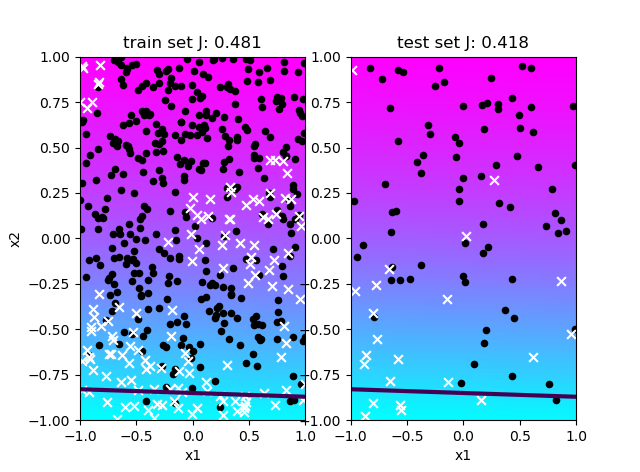
\includegraphics[width=0.5\textwidth]{logreg_deg1_iter20.png}
	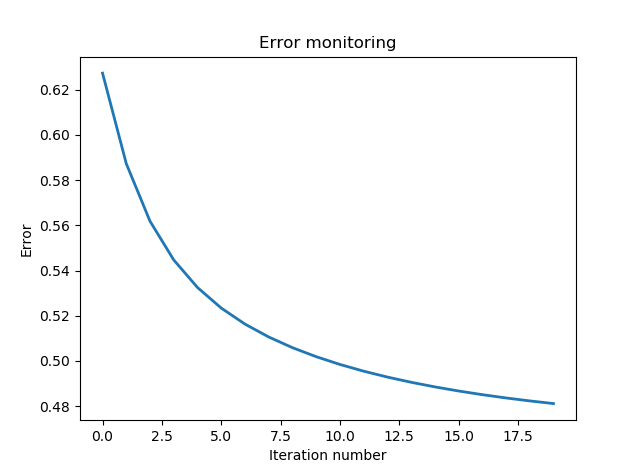
\includegraphics[width=0.5\textwidth]{logreg_deg1_iter20_error.png}
	\caption{iteration = 20}
\end{figure}
\clearpage
\begin{figure}[h]
	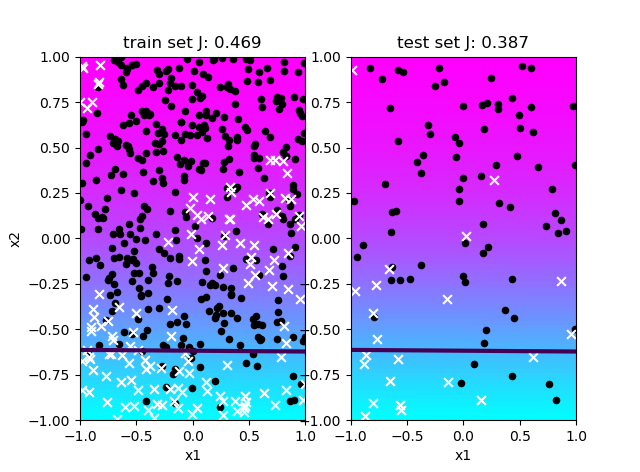
\includegraphics[width=0.5\textwidth]{logreg_deg1_iter2000.png}
	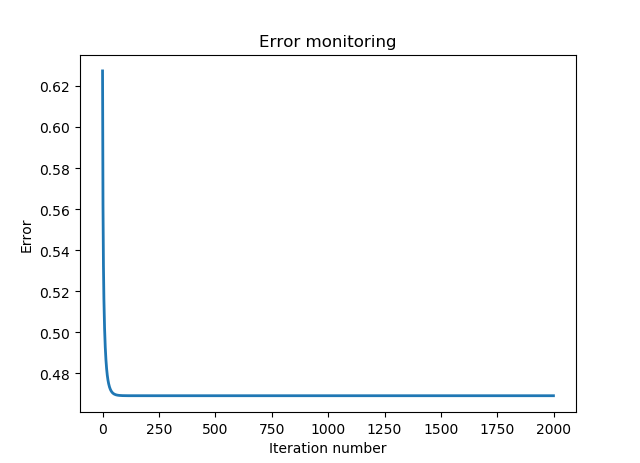
\includegraphics[width=0.5\textwidth]{logreg_deg1_iter2000_error.png}
	\caption{iteration = 2000}
\end{figure}

In the case of figure 1, the process stops before it reaches the local minima. In the case of figure 2, the process reaches the local minima in about 50 iterations. However, it continues to iterate even though the error does not change.

When the number of iterations is too low, the logistic regression process finishes before reaching the local minima.When the number of iterations is too high, it takes a lot of time. Even though it reaches the local minima, it continues to iterate until it reaches the iteration number. Therefore, the number of iterations should not be too low and high.
\paragraph
3 The following plots demonstrate the results of Logistic Regression with degree = 2 , iterations = 200 and learning rate $\eta$ = \{.15, 1.5, 15.\} :
\begin{figure}[h]
	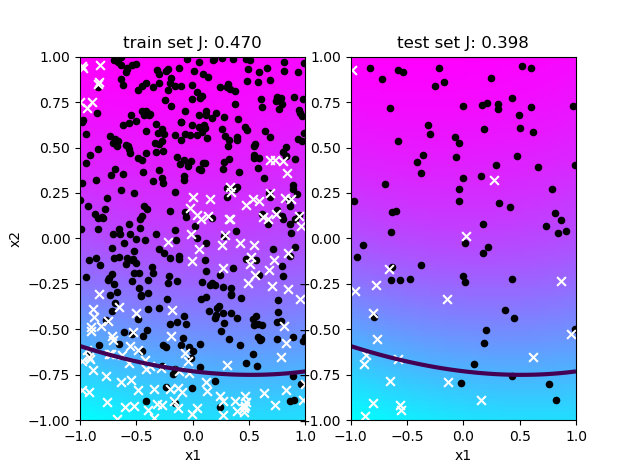
\includegraphics[width=0.5\textwidth]{logreg_deg2_iter200_eta015.png}
	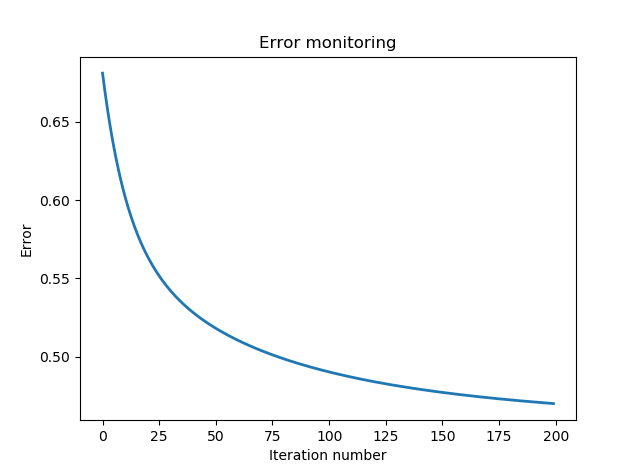
\includegraphics[width=0.5\textwidth]{logreg_deg2_iter200_eta015_error.png}
	\caption{learing rate $\eta$ = .15}
\end{figure}
\clearpage
\begin{figure}[h]
	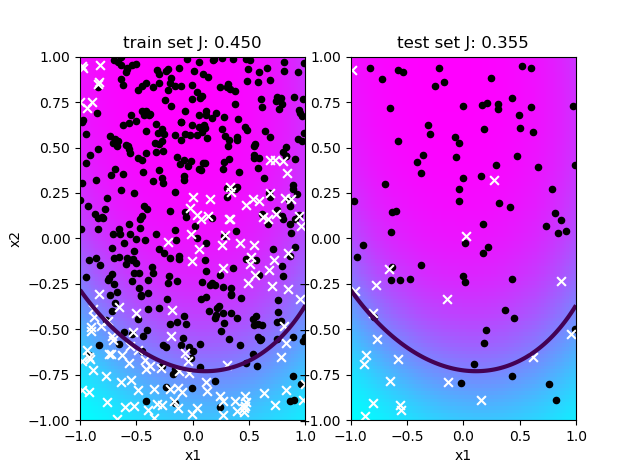
\includegraphics[width=0.5\textwidth]{logreg_deg2_iter200_eta105.png}
	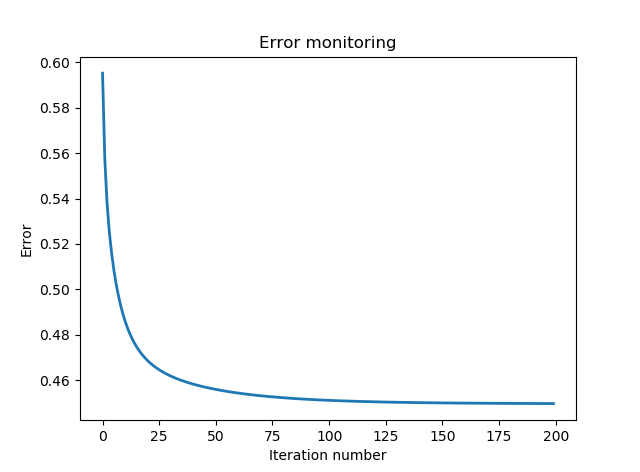
\includegraphics[width=0.5\textwidth]{logreg_deg2_iter200_eta105_error.png}
	\caption{learing rate $\eta$ = 1.5}
\end{figure}
\begin{figure}[h]
	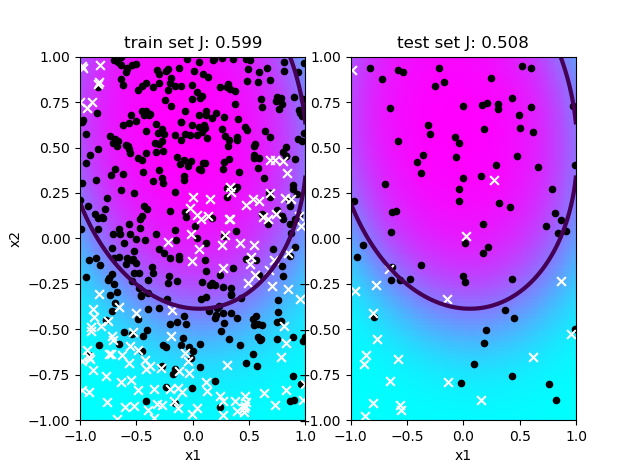
\includegraphics[width=0.5\textwidth]{logreg_deg2_iter200_eta15.png}
	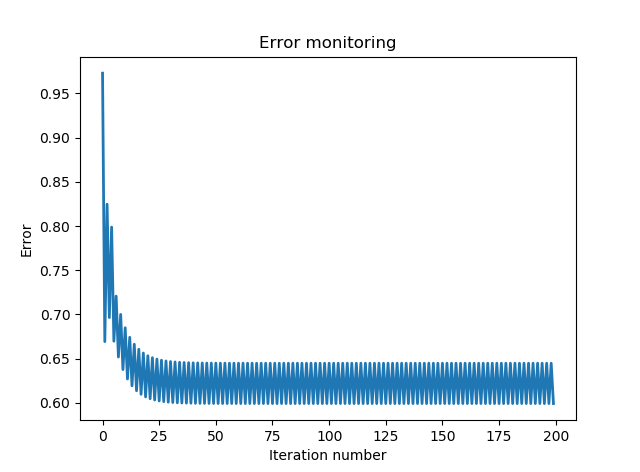
\includegraphics[width=0.5\textwidth]{logreg_deg2_iter200_eta15_error.png}
	\caption{learing rate $\eta$ = 15}
\end{figure}

In the case of figure 3, the process stops before it reaches the local minima. In the case of figure 4, the process reaches the local minima. In the case of figure 5, it doesn't reach the local minima by overshooting the local minima.

When learning rate is too low, it takes a lot of time to reach the local minima or it ends before reaching the local minima. When learning rate is too big, it can overshoot the local minima so it may not reach the local minima or may even diverge.

\paragraph
4
\paragraph
5 One possible way to terminate the gradient descent is setting a threshold to the cost function. While caluating the cost in each iteration, if it is below the setting threshold, it can terminate the process. Using this way, it can not reach the perfect local minima but it can reach close to the local minima depending on the threshold. Therefore it can save time. If high accuracy is aimed, then set the threshold low. And if middle accuracy and high speeed are aimed, then set the threshold a little bit higher.
\subsubsection{Adaptative gradient descent (GDad)}
\paragraph
1 The following plots demonstrate the results of Logistic Regression with iterations = 1000, learning rate $\eta$ = 1 and varying degrees $l$ = \{1, 2, 5, 15\}:

\begin{figure}[h]
	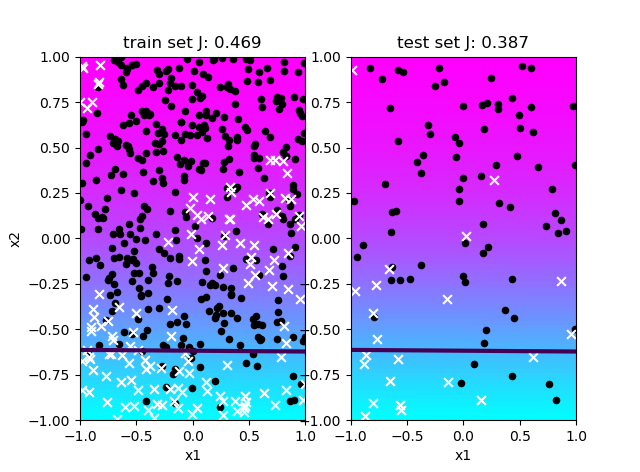
\includegraphics[width=0.4	\textwidth]{logreg_deg1_iter20000.png}
	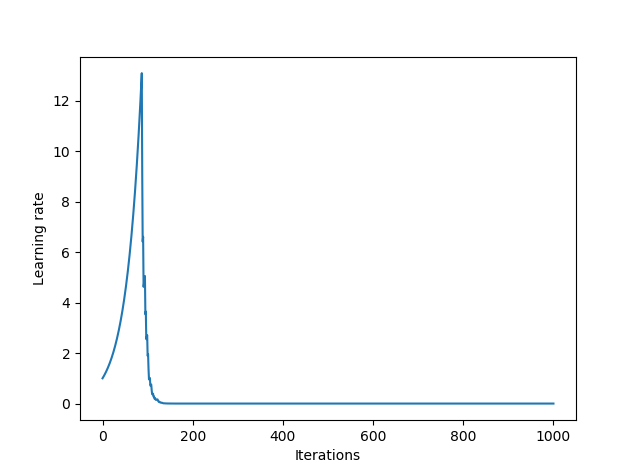
\includegraphics[width=0.4\textwidth]{logreg_deg1_iter20000_learn.png}
	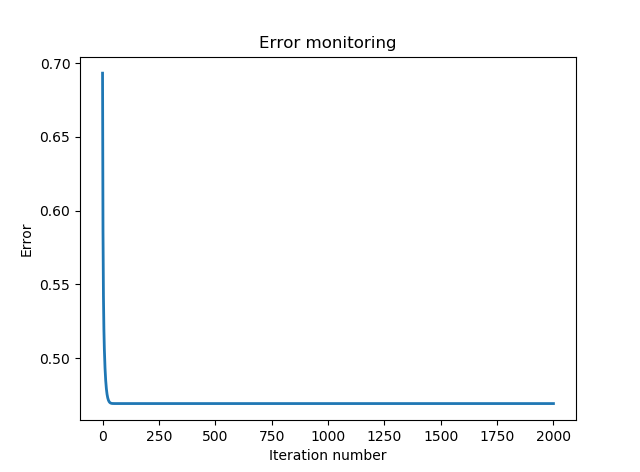
\includegraphics[width=0.4\textwidth]{logreg_deg1_iter20000_error.png}
	\textbf{final learning rate : 2.59$e$\textsuperscript{-132}}
	\caption{degree $l$ = 1}
\end{figure}
	\begin{figure}[h]
	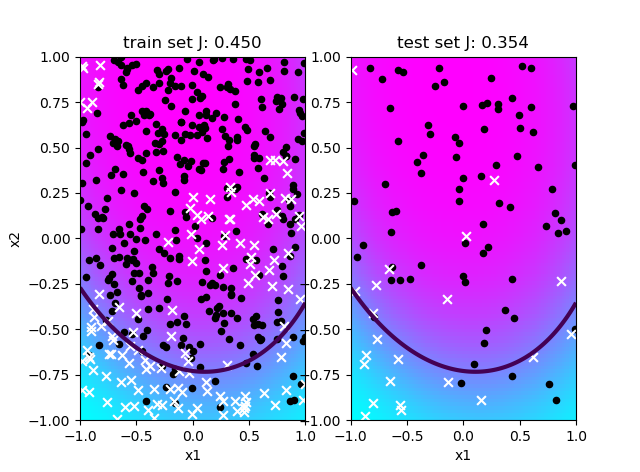
\includegraphics[width=0.4	\textwidth]{logreg_deg2_iter2000.png}
	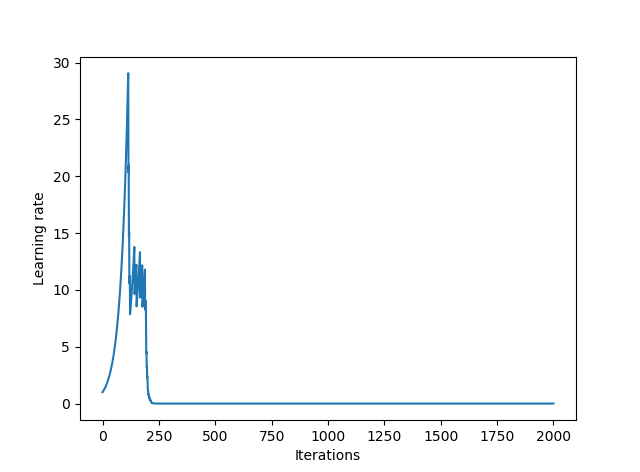
\includegraphics[width=0.4\textwidth]{logreg_deg2_iter2000_learn.png}
	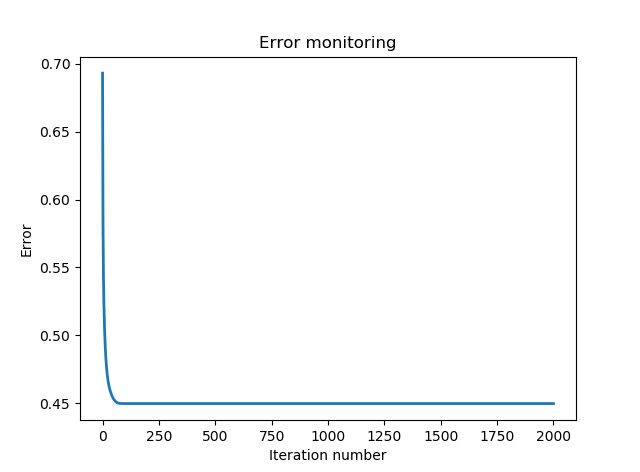
\includegraphics[width=0.4\textwidth]{logreg_deg2_iter2000_error.png}
	\textbf{final learning rate : 3.94$e$\textsuperscript{-274}}
	\caption{degree $l$ = 2}
\end{figure}
\begin{figure}[h]
	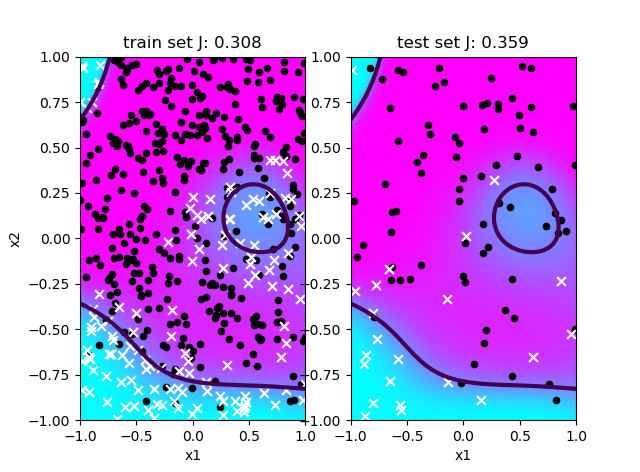
\includegraphics[width=0.4\textwidth]{logreg_deg5_iter2000.png}
	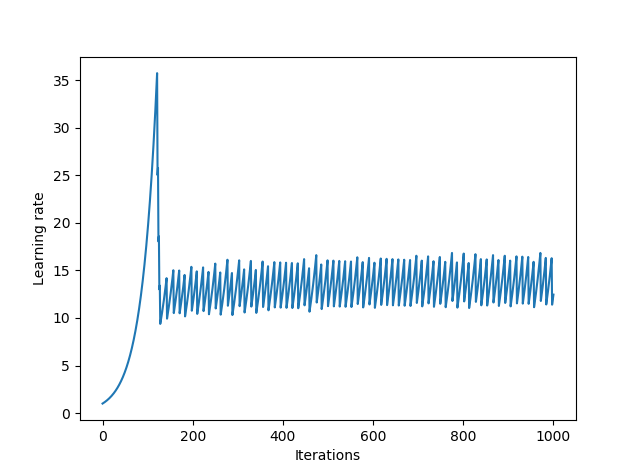
\includegraphics[width=0.4\textwidth]{logreg_deg5_iter2000_learn.png}
	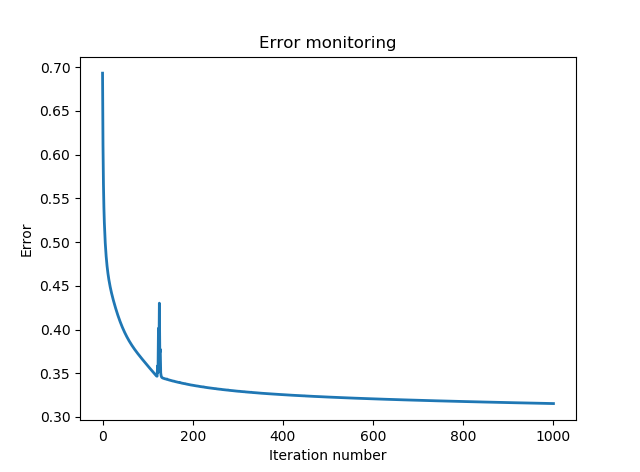
\includegraphics[width=0.4\textwidth]{logreg_deg5_iter2000_error.png}
	\textbf{final learning rate : 12.5}
	\caption{degree $l$ = 5}
\end{figure}
\begin{figure}[h]
	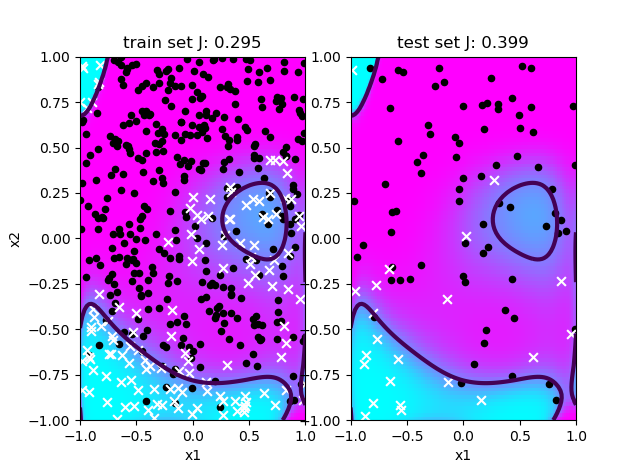
\includegraphics[width=0.4\textwidth]{logreg_deg15_iter2000.png}
	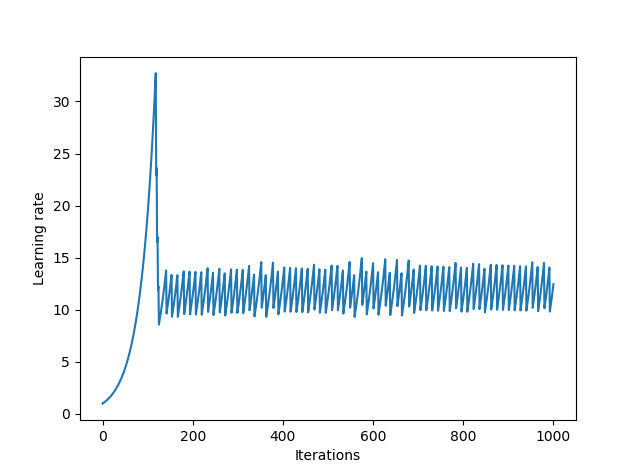
\includegraphics[width=0.4\textwidth]{logreg_deg15_iter2000_learn.png}
	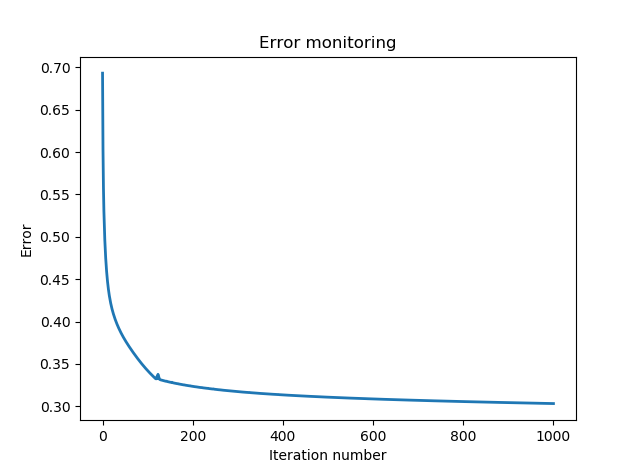
\includegraphics[width=0.4\textwidth]{logreg_deg15_iter2000_error.png}
	\textbf{final learning rate : 12.5}
	\caption{degree $l$ = 15}
\end{figure}
\clearpage
\paragraph
2  These are the comparsion between GDad and non-adpative GD.\\
\textbf{Degree $l$ = 1 :}\\
Speed : GDad reaches near the local minima faster than non-adaptive gradient.\\
Train set error : Both have the same train error(0.469).\\
Test set error : Both have the same test error(0.387).\\
\\
\textbf{Degree $l$ = 2 :}\\
Speed : GDad reaches near the local minima faster than non-adaptive gradient.\\
Train set error : Both have the same train error(0.450).\\
Test set error : Both have the same test error(0.354).\\
\\
\textbf{Degree $l$ = 5 :}\\
Spped : GDad reaches near the local minima faster than non-adaptive gradient.\\
Train set error : GDad have smaller train error(0.315) than non-adaptive GD(0.349).\\
Test set error : GDad have bigger test error(0.353) than non-adaptive GD(0.323).\\
\\
\textbf{Degree $l$ = 15 :}\\
Spped : GDad reaches near the local minima faster than non-adaptive gradient.\\
Train set error : GDad have smaller train error(0.303) than non-adaptive GD(0.333).\\
Test set error : GDad have bigger test error(0.390) than non-adaptive GD(0.342).\\
\\
\\
The evolution of the learning rate is something different from my previous guess of the optimal learning rate. I thought that the evolution of the learning rate looks like a mountain. It is true in the case of degree 1 and 2. However, in the case of degree 5 and 15, the graph vibrates at the latter part because of the overshooting problem.
\\
\\
GDad is more useful than non-adaptive gradient descent in the respect of the speed(when the learning rate is small) and overshooting the minima(when the learning rate is big). \\
First, GDad can reach the local minima faster than non-adaptive gradient descent. When the learning rate is small, gradient descent should iterate more than GDad to reach the local minima. Because, in the case of GDad, the learning rate becomes large when the cost becomes small and can make a big step to the local minima.\\
Second, GDad can avoid the overshooting problem. When the learning rate is big, it can suffer from overshooting problem because the process makes a big step, roams near the local minima and can not reach the local minima. In this case, the costs becomes large and GDad notices that it is in overshooting problem. Then, it can avoid overshooting problem by decreasing the learning rate and reach the local minima. \\
That is, at fist, GDad makes big steps to find the the local minima. Then, when it reaches near the local minima, it decreases the learning rate to avoid the overshooting problem and reachs the local minima.


\subsubsection{Scipy optimizer}
\paragraph
1 The following plots demonstrate the results of Logistic Regression using scipy.optimize, with iterations = 1000, learning rate $\eta$ = 1 and varying degrees $l$ = \{1, 2, 5, 15\}:
\begin{figure}[h]
	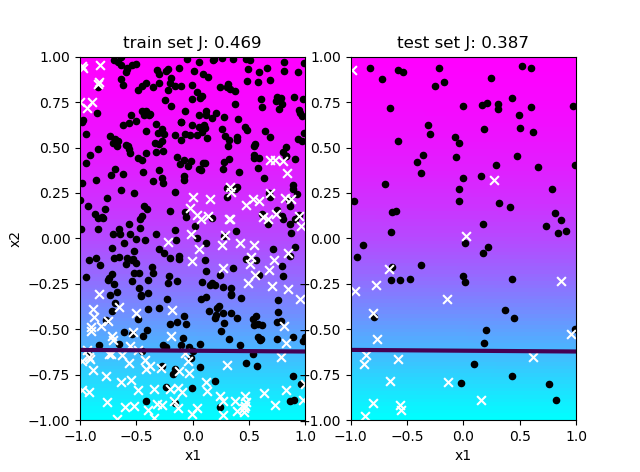
\includegraphics[width=0.4\textwidth]{scipy_1.png}
	\caption{degree $l$ = 1}
	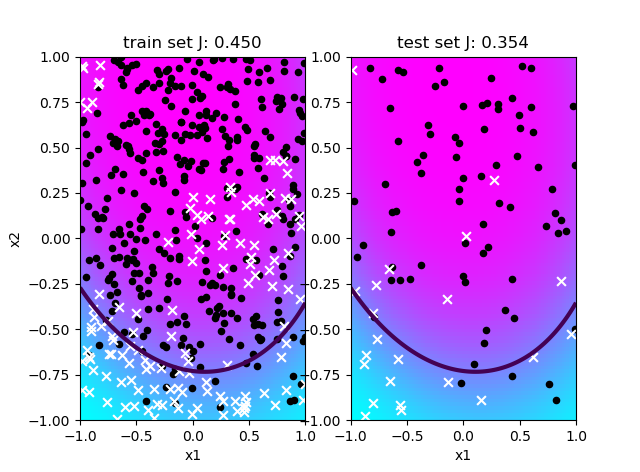
\includegraphics[width=0.4\textwidth]{scipy_2.png}
	\caption{degree $l$ = 2}
	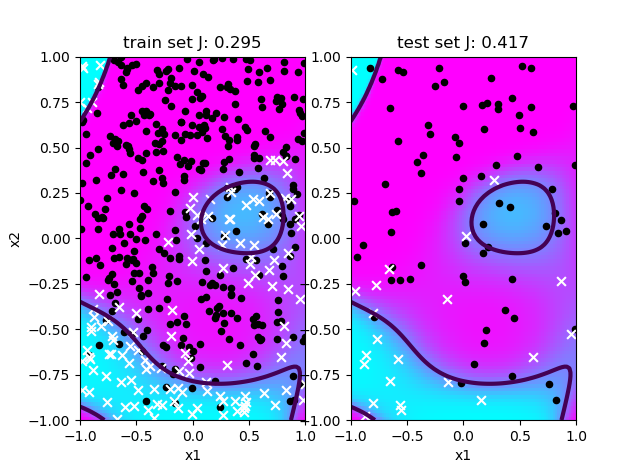
\includegraphics[width=0.4\textwidth]{scipy_5.png}
	\caption{degree $l$ = 5}
	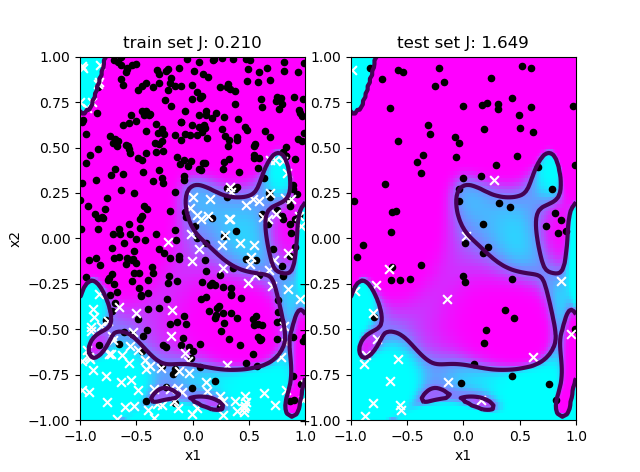
\includegraphics[width=0.4\textwidth]{scipy_15.png}
	\caption{degree $l$ = 15}
\end{figure}
\clearpage

\paragraph
2 These are the comparsion between GDad, non-adpative GD and scipy optimizer.\\
\textbf{Degree $l$ = 1 :}\\
Train set error : All have the same train error(0.469).\\
Test set error : All have the same test error(0.387).\\
\\
\textbf{Degree $l$ = 2 :}\\
Train set error : All have the same train error(0.450).\\
Test set error : All have the same test error(0.354).\\
\\
\textbf{Degree $l$ = 5 :}\\
Train set error : Scipy optimizer(0.295) $<$ GDad (0.315) $<$ GD(0.349).\\
Test set error : Scipy optimizer(0.417) $>$ GDad(0.353) $>$ GD(0.323).\\
\\
\textbf{Degree $l$ = 15 :}\\
Train set error : Scipy optimizer(0.210) $<$ GDad(0.303) $<$ GD(0.333).\\
Test set error : Scipy optimizer(1.649) $<$ GDad (0.390) $<$ non-adaptive GD(0.342).\\
\\
Scipy optimizer optimizes the cost function better than the others. Therefore it has the lowest train set errors in all degrees. However, it has the highest test set error in all degrees. I think it is becuase of overfitting to the train set. Scipy optimizer makes a hypothesis fit perfectly to train set so it causes overfitting problem and get the highest test set error.\\
\\
It doesn't change my opinion that degree $l$ = 5 is best to fit the data. Low degree can not predict the complex hypothesis and high degree can cause the overfitting problem. Therfore, appropriate degree is the best. In this problem, it is 5.

\end{document}
